%\begin{relatedwork}

% add chapter to table of contents
%\addchaptertocentry{Related Work}

\chapter{Related work}

\section{C\# nameof}

    C\# has a \texttt{nameof} expression that is used to obtain the name of a program element as a constant string.\footnote{\href{https://docs.microsoft.com/en-us/dotnet/csharp/language-reference/operators/nameof}{\texttt{nameof}}} 

\begin{minted}{csharp}
using System.Collections.Generic;

class Program {
    static void Main() {
        string s1 = nameof(Program);                     // "Program"
        string s2 = nameof(Program.InstanceMethod);      // "InstanceMethod"
        string s3 = nameof(System.Collections.Generic);  // "Generic"
        // Invalid
        string s4 = nameof(int);               // Keywords not permitted
    }
    void InstanceMethod() { }
}
\end{minted}

% TODO
The result of the \texttt{nameof} expression is evaluated at compile time, meaning that \texttt{nameof(x)} if \texttt{x} is legal input is replaced by \texttt{"x"} in the resulting bytecode of the program. Our interest is drawn, however, to the use of property literals as string constants. And indeed nameof accepts class properties as input:

\begin{minted}{csharp}
class Book {
    public string title { get; set; }
}
nameof(Book.title) // "title"
\end{minted}

This is quite an effective way of using property literals as constant strings and it satisfies the compile time model correctness property. There are, however, several limitations to this approach, which are demonstrated below with provided examples:

\begin{enumerate}
    \item The \texttt{nameof} expression cannot be applied to class members with restricted access, such as private members. Although we consider this a limitation, the example above, which makes use of C\# Properties\footnote{\href{https://docs.microsoft.com/en-us/dotnet/csharp/programming-guide/classes-and-structs/properties}{C\# properties}}, is not constrained by it.

    \item The nameof expression always returns a simple name of its input, that is, the resulting name is not fully-qualified. This was demonstrated in the first code snippet:
\begin{minted}{csharp}
    string s3 = nameof(System.Collections.Generic);  // "Generic"
\end{minted}

\end{enumerate}

This limitation requires additional functionality to be implemented to concatenate the resulting string constants into a proper representation of the dot-notation.

\begin{minted}{csharp}
class Book {
    public string title { get; set; }
    public Author author { get; set; };
}
class Author {
    public string fullName { get; set; }
}

// "author.fullName"
DotNotation.Of(nameof(Book.author), nameof(Book.author.fullName));

class DotNotation {
    public static string Of(params string[] names) {
            return String.Join(".", names);
    }
}
\end{minted}

\texttt{Book.author.fullName} is used instead of simply \texttt{Author.fullName} to satisfy the compile time safety requirement. If the latter was used and the conceptual schema was changed leading to the type of \texttt{Book.author} not being \texttt{Author} anymore, but instead a value object or another entity that doesn’t have the property \texttt{fullName}, a run-time error would occur at the moment of the dot-notation being used (to fetch some data from a database, for example). Consequently, this results in an unintuitive and overly verbose code.

\section{Java nameof hack}

While the java programming language specification does not define property literals or an expression similar to that of C\# \texttt{nameof}, there are 3rd party libraries that attempt to achieve the desired result by means of byte-code manipulation through the use of method references.\footnote{\href{https://github.com/strangeway-org/nameof}{nameof by strangeway-org}

\; \; \href{https://github.com/mobiuscode-de/nameof}{nameof by mobiuscode-de}}


\subsection{Method references}
Java has a special syntax for referring to a method of a class as if it was a lambda expression. Consider the following example: 

\begin{minted}{java}
class Person {
    private String name;
    public String getName() {
        return this.name;
    }
}
\end{minted}

This makes it possible to avoid writing a full lambda expression:
\begin{minted}{java}
    map(person -> person.getName()); // lambda expression
    map(Person::getName);            // method reference
\end{minted}

\subsection{Reflection and byte-code manipulation}
Reflection is a feature in the Java programming language that allows a Java program to discover and manipulate information about itself in the runtime. More precisely, one can obtain information such as names of class members, their types, etc. In addition, it is possible to "intercept" a method of a class by using a \textit{dynamic proxy}. In this case an interceptor would gain access to the information about the intercepted method, such as its name, parameter types, return type, etc.

\subsection{The hack}
The idea is to use a combination of method references and reflection to intercept the getter method call, such as \texttt{getName()} in the above example and map the method name to a field name, for which the getter was designed. As a result it would be possible to get the property name as a String in a compile time safe manner:

\begin{minted}{java}
nameOf(Person.class, Person::getName) // "name"
\end{minted}

As this approach is merely mimicking the \texttt{nameof} expression of C\#, it is subject to the same limitations. In addition, there is no way of chaining properties to construct a dot-notation in a compile time safe manner, since method references are semantically equivalent to lambda expressions.

\section{Project Lombok}
Project Lombok provides a handful of useful additions to the java programming language in the form of annotations with the aim to reduce boilerplate code (footnote). The specificity of this approach lies in the fact that lombok injects itself into the compilation phase to build on top of the source code being compiled, that is, lombok’s annotations are used to replace repetitive pieces of code.

\n

Project Lombok makes use of annotation processing for the sole purpose of identifying the supported annotations, i.e., as an entry point, and, unlike the original purpose of APT, does not generate any source files. Instead it uses the internal API of java compiler (supports javac and ecj\footnote{Eclipse Compiler for Java}) to manipulate the AST. The resulting AST is then analyzed and translated into bytecode.
\begin{figure}[ht]\centering
    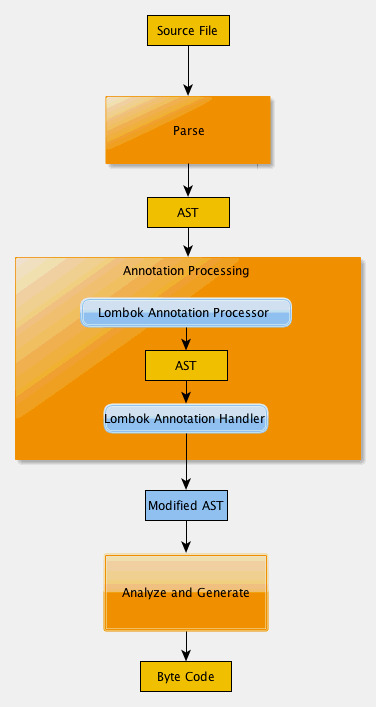
\includegraphics[scale=0.5]{images/lombok.jpg}
    \caption{Lombok Annotation Processor modifies the AST}
    \label{fig:lombok}
\end{figure}

\subsection{@FieldNameConstants annotation}
One of the experimental features of Project Lombok, \texttt{@FieldNameConstants}\footnote{\url{https://projectlombok.org/features/experimental/FieldNameConstants}} annotation is used to generate an inner type that contains a string constant representing a field’s name for each field of the annotated type. This annotation is provided with some room for configuration, such as inclusion or exclusion of particular fields, capitalization of generated fields names, the name of the inner generated type, etc.

Java source with Lombok:
\begin{minted}{java}
@FieldNameConstants
public class Person {
    private String name;
    private int age;
    @FieldNameConstants.Exclude
    private String id;
}
\end{minted}

Equivalent Java source without Lombok:
\begin{minted}{java}
public class Person {
    private String name;
    private int age;
    private String id;

    public static final class Fields {
        public static final String name = "name";
        public static final String age = "age";
    }
}
\end{minted}

This approach, although effective for basic needs, is limited by its simplicity, as indicated by the following points:
\begin{itemize}
    \item The generated entity graph is limited by a depth of a single level, as the generated fields are always of type String.
    \item Domain discoverability is limited by the lack of descriptiveness of the generated fields, since no javadoc accompanying a field is generated.
\end{itemize}

However, the approach employed by Project Lombok is certainly a unique and inspiring piece of work to learn from.

\section{Hibernate Metamodel Generator}

Hibernate is an implementation for the JPA\footnote{Java Persistence API (renamed to Jakarta Persistence)}.

\n

Hibernate Metamodel Generator\footnote{\url{https://docs.jboss.org/hibernate/orm/6.0/topical/html\_single/metamodelgen/MetamodelGenerator.html}} is an annotation processing tool that is a part of the Hibernate ORM framework. It automates the generation of static entity meta-models used for typesafe Criteria queries as defined by the JPA 2. The queries benefit from the meta-models by being able to be constructed in a strongly-typed manner, thus avoiding the risks of type casting the result of a query.

\begin{minted}{java}
@Entity
public class Order {
    @Id
    private long id;

    @ManyToOne
    private Person customer;

    @OneToMany
    private Set<Item> items;

    private BigDecimal totalCost;
}

@StaticMetamodel(Order.class)
public abstract class Order_ {

    public static volatile SingularAttribute<Order, Long> id;
    public static volatile SetAttribute<Order, Item> items;
    public static volatile SingularAttribute<Order, BigDecimal> totalCost;
    public static volatile SingularAttribute<Order, Person> customer;

    public static final String ID = "id";
    public static final String ITEMS = "items";
    public static final String TOTAL_COST = "totalCost";
    public static final String CUSTOMER = "customer";

}

\end{minted}

What stands out is that, apart from the property names, the generated meta-model also captures information about property types, providing an ability to use them in a compile time safe manner. However, since this tool was specifically designed to assist with constructing Criteria queries, its area of application is to some extent bound to the JPA specifications. More specifically, those members of the generated meta-model that capture the property type as a generic type parameter (the first four in the example) are a part of the JPA, hence the tightly coupled implementation.

\n

The major limitation of Hibernate meta-models is that their use for other, JPA unrelated, purposes will most likely end up being as effective as the previously mentioned approach of Project Lombok, thus being subject to the same constraints.


%\end{relatedwork}
